\documentclass{beamer}[10]
\usepackage{pgf}
\usepackage[danish]{babel}
\usepackage[utf8]{inputenc}
\usepackage{beamerthemesplit}
\usepackage{graphics,epsfig, subfigure}
\usepackage{url}
\usepackage{srcltx}
\usepackage{hyperref}
\usepackage{verbatim} 
\usepackage{lmodern}

\definecolor{kugreen}{rgb}{0.0, 0.2, 0.13}
%\definecolor{kugreen}{RGB}{50,93,61}
\definecolor{kugreenlys}{RGB}{132,158,139}
\definecolor{kugreenlyslys}{RGB}{173,190,177}
\definecolor{kugreenlyslyslys}{RGB}{214,223,216}
\setbeamercovered{transparent}
\mode<presentation>
\usetheme[numbers,totalnumber,compress,sidebarshades]{PaloAlto}
\setbeamertemplate{footline}[frame number]

  \usecolortheme[named=kugreen]{structure}
  \useinnertheme{circles}
  \usefonttheme[onlymath]{serif}
  \setbeamercovered{transparent}
  \setbeamertemplate{blocks}[rounded][shadow=true]

\logo{
\includegraphics[width=1.5cm,height=1.5cm]{logo}}
%\useoutertheme{infolines} 
\title{Brain Fiber Segmentation}
\author{Anand K. Parmar  B12021\\ Mani Kumar \hspace{0.7cm} B12012 \newline \newline Mentor\\Dr. Aditya Nigam}
\institute{School of Computing and Electrical Engineering \\ Indian Institute of Technology, Mandi}
\date{09 Oct, 2015}



\begin{document}
\frame{\titlepage \vspace{-0.5cm}
}

\frame
{
\frametitle{Index}
\tableofcontents%[pausesection]
}

\section{Problem Statement}

\frame{
\frametitle{Problem Statement and Long Term Goal}
\begin{block}{Problem Statement}
\setlength{\parindent}{5ex} Given the tractography data of a human brain, Segment it
automatically into tracts having \textbf{"similar"} fibers which are
anatomically meaningful.
\end{block}
\begin{block}{Goal}
\setlength{\parindent}{5ex} Make a software, which will take tractography data of brain as input and gives "similar" fiber 3D model of brain and some useful information according to given application( like, for brain tumor operation, it will give us shortest path for cutting fibers to remove tumor.)  
\end{block}
}


\frame{
\frametitle{Problem Statement and Long Term Goal}
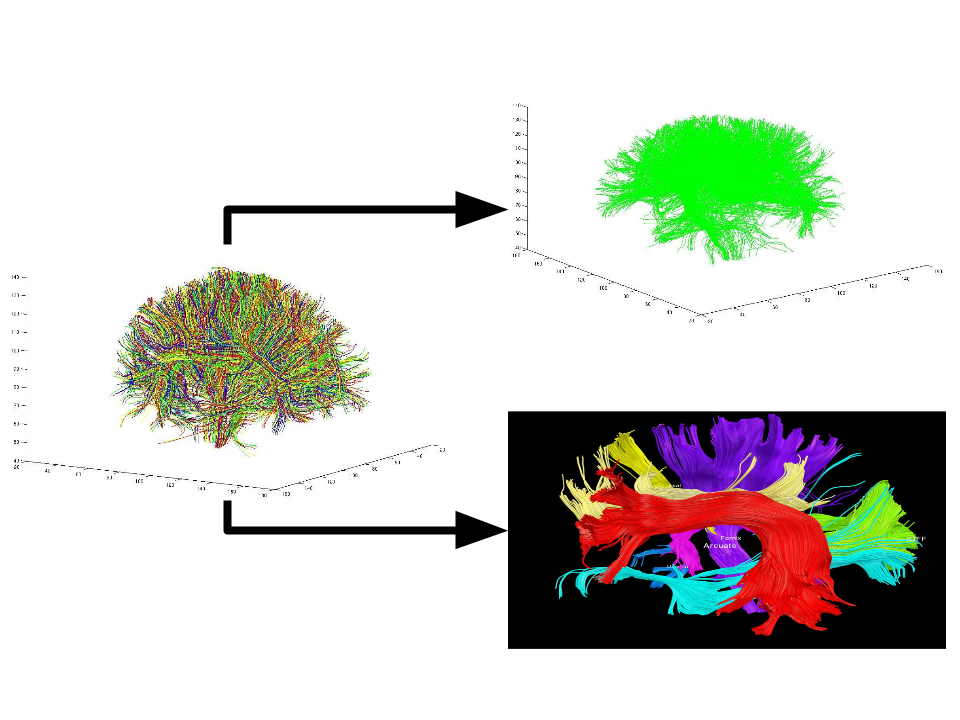
\includegraphics[width=10cm,height=7cm]{goal}
}

\section{Motivation}

\frame
{
\frametitle{Motivation}
\begin{center}
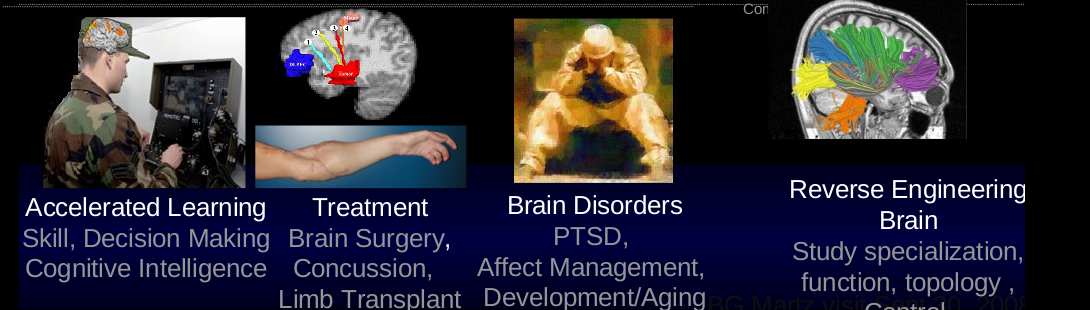
\includegraphics[width=10cm,height=4cm]{applications}
\end{center}
\begin{itemize}
\item To Study about the localization of specific tracks of fibers.
\item Surgery planning with minimum damage to the fibers.
\end{itemize}
}

\section{Background}

\frame{
\frametitle{Background and Related Work}
\begin{itemize}
	\item White matter atlas creation, using group spectral clustering of tractography and Automatic Segmentation of Tractography from novel subjects by extending the spectral clustering solution, stored in the atlas, using the Nystrom Method. (Donnell-Westin, 2007)
	\item Treating image segmentation as a graph partitioning problem and proposing novel global criterion, the normalized cut, for segmenting the graph.(Shi and Malik, 2000)
	\item Proposing a nonparametric Bayesian framework to cluster white matter fiber tracts into bundles using a hierarchical Dirichlet Processes Mixture(HDPM) Model.  (Wang-Eric-Westin, - )
\end{itemize}
}

\section{Introduction}

\frame{
\frametitle{Introduction}
\begin{itemize}
\item The brain contains more than 100 billion neurons that communicate with each other via axons for the formation of complex neural networks.
\item In Brain, two kinds of tissue are there: 
	\begin{itemize}
	\item Grey matter,
	\item White matter.
	\end{itemize}  
\end{itemize}
}

\frame{
\frametitle{Introduction: Brain}
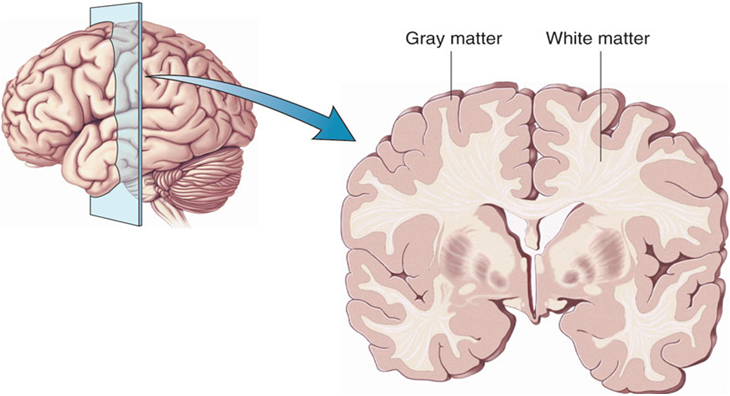
\includegraphics[width=10cm,height=5cm]{Brain_Cortex_Harvard}
\begin{itemize}
	\item Grey matter, which has a pinkish-grey color in the living brain, contains the cell bodies, dendrites and axon terminals of neurons, so it is where all synapses are. 
	\item White matter is made of axons connecting different 	parts of grey matter to each other.
\end{itemize}
}

\frame{
\frametitle{Introduction: Neuronal cell Structure}
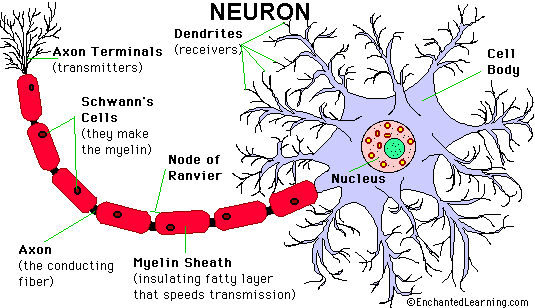
\includegraphics[width=10cm,height=5cm]{Neuron}
}

\frame{
\frametitle{Introduction: Communication in Neurons}
\begin{center}
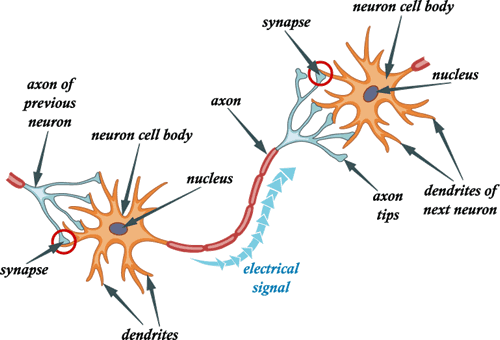
\includegraphics[width=7cm,height=3.5cm]{Neuron_connection}
\end{center}
 Here, Dendrites receives signals from other neurons, the cell body, which processes those signals and the axon, a long cable that reaches out and interacts with other neuron’s dendrites. When different parts of the brain communicate and coordinate with each other, they send nerve impulses, which are electrical charges that travel down the axon of a neuron, eventually reaching the next neuron in the chain.
}

\section{Brain Data}

\subsection{Data collection process}

\frame{
\frametitle{Diffusion Tensor Imaging(DTI)}
\begin{itemize}
\item It is important when a tissue, such as the neural axons of white matter in the brain has an internal anisotropy fibrous structure.
\item Water will then diffuse more rapidly in the direction aligned with the internal structure, and more slowly as it moves perpendicular to the preferred direction.
\item Tensors are used to model diffusion. Major eigen vectors of the tensor(Principle Directions) gives the fiber tract direction.
\begin{center}
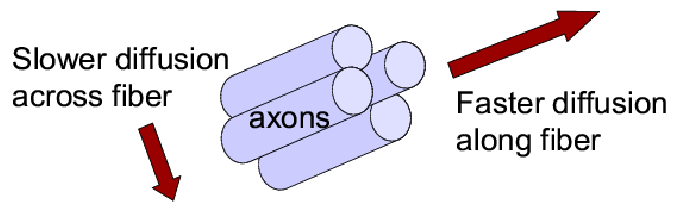
\includegraphics[width=7cm,height=3cm]{diff2}
\end{center}
\end{itemize}
}

\frame{
\frametitle{Tractography}
\begin{block}{wikipedia.org}
In neuroscience, tractography is a 3D modeling technique used to visually represent neural tracts using data collected by diffusion tensor imaging (DTI).
\end{block}
\begin{itemize}
\item Streamline Tractography estimates white matter tract trajectories
following the most likely tract direction. It locally chooses the most
likely fiber trajectory.
\item \textbf{DTI with Tractography gives us the white matter fiber orientation.}
\end{itemize}
}

\frame{
\frametitle{Tractography}
\begin{center}
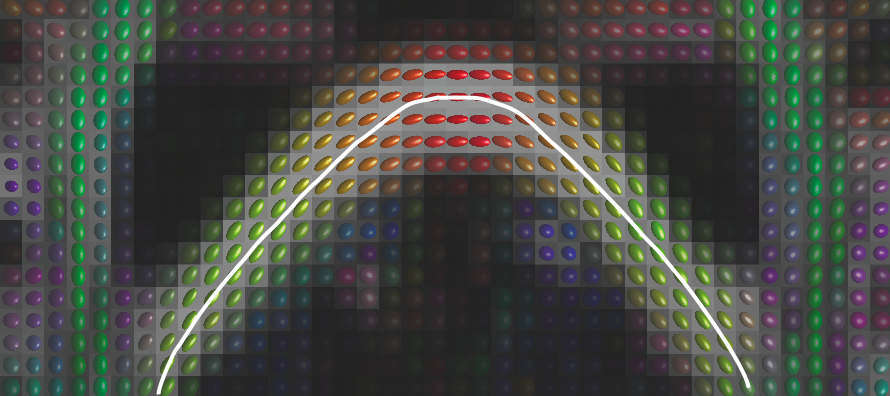
\includegraphics[width=10cm, height=4cm]{tractography-fig1}
\end{center}
Preferred diffusion directions are shown as the long axes of diffusion ellipsoids.Here, red denotes left-right, green denotes back-front and blue up-down direction(out of the image plane). The white line shows the streamline obtained by connecting up a set of pixels based on their preferred directions and is an example of tractography.
}

\subsection{Data Format}

\frame{
\frametitle{Available data with us}
Initially, we have 3 brain’s data as .trk file format.
\begin{itemize}
\item brain’s data (classified) which is ground truth model for us. 
\item brain’s data (Non-classified) which can be used for testing.
\end{itemize}
}


\frame{
\frametitle{Data Format}
	The data is given in a file with .trk extension. Track(.trk) file is one single binary file, with the first 1000 bytes as the header and rest as the body. Some fields of header of track file are-
\begin{center}
\begin{tabular}{ |l|l|l| }
  \hline
  \textbf{Name} & \textbf{Data-type} & \textbf{Bytes} \\
  \hline
  id\_string[6] & \textit{char} & 6 \\
  dim[3] & \textit{short int} & 6 \\
  voxel\_size[3] & \textit{float} & 12 \\
  n\_count & \textit{int} & 4 \\
  version & \textit{int} & 4\\
  hdr\_size & \textit{int} & 4\\
  
  \hline
\end{tabular}
\end{center}

 
And the body part of the file contains $"n\_count"$ numbers of fibers as struct type and each struct of fiber contains \textbf{1.num\_points}: number of points in that fiber, \textbf{2. 2D array} of num\_point * 3, 
where each row displays x, y, z coordinates of points of that fiber.

	
}

\frame{
\frametitle{Note}
Here, we are using some name for particular things, which are mentioned below:
\begin{itemize}
\item Ground truth data - Brain1 data (classified)
\item Class 0 - Grey Matter of Brain
\item Classes of white matter fiber tracts:
\end{itemize}
\begin{center}
\begin{tabular}{ |l|l| }
  \hline
  \textbf{Class no.} & \textbf{Class Name} \\
  \hline
  Class1 & Arcuate \\
  Class2 & Cingulum \\
  Class3 & Corticospinal \\
  Class4 & Forceps Major \\
  Class5 & Fornix \\
  Class6 & Inferior Occipitofrontal Fasciculus \\
  Class7 & Superior Longitudinal Fasciculus \\
  Class8 & Uncinate\\
  \hline
\end{tabular}
\end{center}
}


\section{Results}

\frame{
\frametitle{Result(1)}
\begin{tabular}{ |l|l| }
  \hline
  \textbf{Class no.} & \textbf{Start-points Mean} \\
  \hline
  Class1 & (41.75930000,132.90225000,97.68317000) \\
  Class2 & (78.09513500,136.08315000,103.33668500) \\
  Class3 & (90.27637500,91.59677500,42.43649000) \\
  Class4 & (79.32306000,42.33381500,80.40204000) \\
  Class5 & (89.58828500,113.84820000,64.95563500) \\
  Class6 & (74.16783000,143.52725000,70.49763500) \\
  Class7 & (49.87368500,127.74495000,118.32490000) \\
  Class8 & (113.37985000,132.37805000,51.36863000) \\
  \hline
\end{tabular}
}

\frame{
\frametitle{Result(2)}
\begin{tabular}{ |l|l| }
  \hline
  \textbf{Class no.} & \textbf{Start-points Standard deviation} \\
  \hline
  Class1 &  (3.59007200,1.65377037,2.55151559) \\
  Class2 &  (4.80101352,6.46182409,2.89388383) \\
  Class3 &  (0.18937435,0.47351493,0.22717374) \\
  Class4 &  (5.34165247,3.08654294,2.31996886) \\
  Class5 &  (2.22060831,1.51108827,1.66560462) \\
  Class6 &  (3.34551431,7.42975410,14.83555032) \\
  Class7 &  (0.39485908,0.52277337,0.41652010) \\
  Class8 &  (4.39531984,4.82689752,10.91509012) \\
  \hline
\end{tabular}
}


\frame{
\frametitle{Result(3)}
\begin{tabular}{ |l|l| }
  \hline
  \textbf{Class no.} & \textbf{End-points Mean} \\
  \hline
  Class1 & (40.06050500,70.78955500,67.03863500) \\
  Class2 & (80.37367000,74.72157500,97.63405500) \\
  Class3 & (113.63880000,93.41260500,131.96160000) \\
  Class4 & (94.92560000,43.25754500,85.80602500) \\
  Class5 & (99.47859000,89.79473000,87.79484500) \\
  Class6 & (71.82542500,46.68512000,71.95375500) \\
  Class7 & (55.48636000,61.11233000,112.44245000) \\
  Class8 & (110.58140000,127.81460000,61.19712000) \\
  \hline
\end{tabular}
}

\frame{
\frametitle{Result(4)}
\begin{tabular}{ |l|l| }
  \hline
  \textbf{Class no.} & \textbf{End-points Standard deviation} \\
  \hline
  Class1 & (2.92963392,3.72654027,1.47660720) \\
  Class2 & (2.84154346,2.92655120,6.99558243) \\
  Class3 & (1.25299823,1.39776723,0.56241572) \\
  Class4 & (5.78067766,3.68521876,8.15535096) \\
  Class5 & (7.50444281,6.03372304,2.54777244) \\
  Class6 & (3.05448935,4.78675452,5.94266455) \\
  Class7 & (2.08037457,1.94918669,1.98636540) \\
  Class8 & (3.92595123,3.12721375,8.44942414) \\
  \hline
\end{tabular}
}

\frame{
\frametitle{Result(5)}
\begin{tabular}{ |l|l|l| }
  \hline
  \textbf{Class no.} & \textbf{Mean Length} & \textbf{Standard deviation} \\
  \hline
  Class0 & 63.2312441493006 & 28.6485729787890 \\
  Class1 & 90.6890004417171 & 13.1847545751457  \\
  Class2 & 61.1771305385634 & 17.7718004108051 \\
  Class3 & 83.7487559847006 & 18.2878480190662 \\
  Class4 & 120.422320606324 & 9.34715491299375 \\
  Class5 & 39.9237420331200 & 11.8112475345795 \\
  Class6 & 119.862410788331 & 14.6056708300016 \\
  Class7 & 81.8378630440721 & 13.7995291380608 \\
  Class8 & 36.4855790683932 & 6.96950091496981 \\
  \hline
\end{tabular}
}

\frame{
\frametitle{Result(6)}
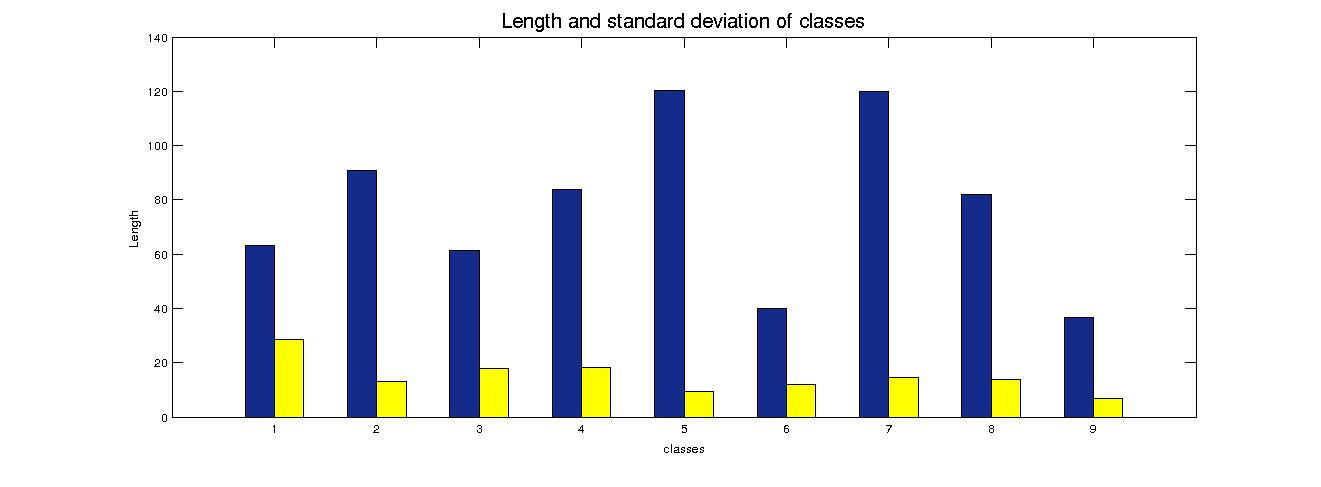
\includegraphics[width=10cm,height=6cm]{length_chart}

}

\frame{
\frametitle{Working on}
\begin{itemize}
\item Here, by observations we can say that above 105, we have only two classes eg. class-4 and class-6. So we can consider that point to classify this two class from rest of data.
\item Also we are observing starting and ending points of classes as well as curvature points of classes for classification.
\end{itemize}
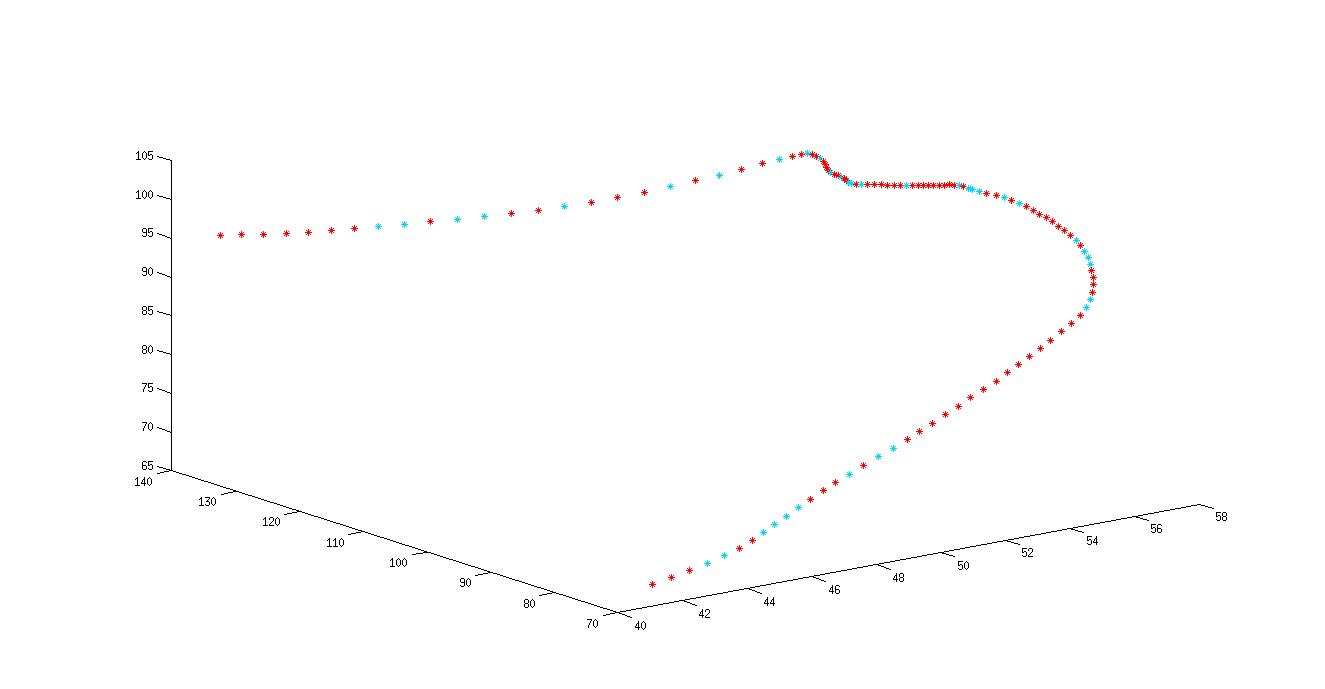
\includegraphics[width=10cm,height=6cm]{curvature_point1}

}

\section{Gantt chart}

\frame{
\frametitle{Gantt chart}
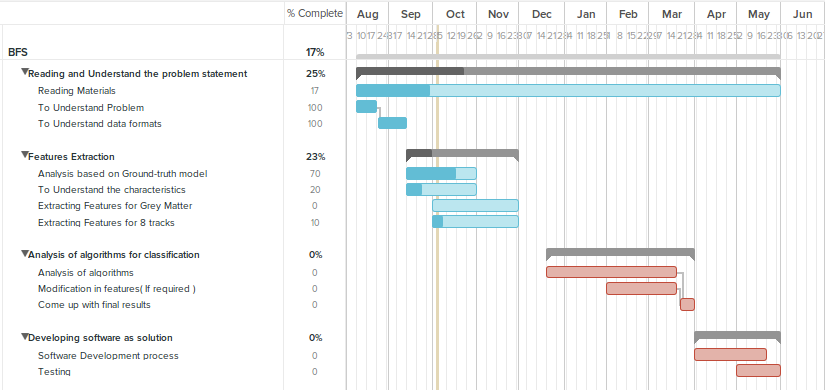
\includegraphics[width=10cm,height=6cm]{gantt}
}



\section{References}

\frame{
\frametitle{References}
\begin{itemize}
\item \url{wikipedia.com}
\item \url{www.lrdc.pitt.edu/schneider/bcm/}
\item \url{www.trackvis.org/docs/?subsect=fileformat}
\item Lauren J. O’Donnell and Carl-Fredrik Westin (2007). \textbf{\textit{Automatic Tractography Segmentation Using a High Dimensional White Matter Atlas}} . Members, IEEE \\ \textbf{In-text Reference:} (Donnell-Westin, 2007)
\item Jianbo Shi and Jitendra Malik(2000). \textbf{\textit{Normalized Cuts and Image Segmentation}}.Members, IEEE \\ \textbf{In-text Reference:} (Shi and Malik, 2000)
\item Xiaogang Wang, W. Eric L. Grimson and Carl-Fredrik Westin.\textbf{\textit{Tractography	Segmentation using a Hierarchical Dirichlet Processes Mixture Model}}. \\ \textbf{In-text Reference:} (Wang-Eric-Westin, - )
\end{itemize}
}

%%%%%%%%%%%%%%%
\begin{comment}
\frame{
\frametitle{References Cont...}

}
\end{comment}
%%%%%%%%%%%%%%%

\frame{
\frametitle{Thank You}
}

\end{document}
